\subsubsection{Galvanic skin reaction and temperature data;}
\label{subsubsec:results_gsr_temp_2}

The GSR analysis is made by analyzing its average and the accumulated value and comparing both features between the baseline and each round. The temperature was analyzed with the GSR to see if there is some influence and by a graphical analysis there was none. For the experiment, the GSR sensor was worn on the left hand for right-handed participant and on the right hand for left-handed participants.

The Table \ref{tab:gsr_table_blind} presents the standard deviation of the interbeat interval by each participant on each scenes. As it was with the Table \ref{tab:bpm_table_blind}, it is not posible to draw a pattern inside this Table. Different participant had increase, or decrease, with different methods.


The Table \ref{tab:gsr_table_blind} presents the average skin conductance by each blind participant on their baseline and on each scene and their respectivily variation is inside Table \ref{tab:gsr_var_blind}. In the majority of times the skin conductance has risen from the "First" to the "Return" round, which mean that the participant was more aroused or with a higher mental workload.


\begin{table}[!htb]
\centering
\caption{Average GSR felled by the blind participants [$\mu$S].}
\label{tab:gsr_table_blind}
\begin{tabular}{lllrrrrrr}
\toprule
     &        & Baseline &  Base & Audio & \begin{tabular}[c]{@{}l@{}}Haptic\\ Belt\end{tabular} & \begin{tabular}[c]{@{}l@{}}Virtual\\ Cane\end{tabular} & Mixture \\
Participant & Round &          &       &       &                                                       &                                                        &         \\
\midrule
001C & First &     0.37 &  0.48 &  1.03 &                                                  3.14 &                                                   3.79 &    3.90 \\
     & Return &          &  0.83 &  1.58 &                                                  2.81 &                                                   4.04 &    4.57 \\
003C & First &     0.30 &  0.56 &  0.56 &                                                  0.62 &                                                   0.85 &    1.09 \\
     & Return &          &  0.62 &  0.63 &                                                  0.65 &                                                   0.92 &    1.06 \\
004C & First &     1.24 &  2.34 &  3.07 &                                                  3.49 &                                                   2.28 &    2.23 \\
     & Return &          &  2.57 &  2.95 &                                                  3.20 &                                                   2.21 &    2.24 \\
\bottomrule
\end{tabular}
\end{table}




\begin{table}[!htb]
\centering
\caption{Average GSR variation in relation to the baseline in each round of the blind participants [$\mu$S].}
\label{tab:gsr_var_blind}
\begin{tabular}{lllrrrrrr}
\toprule
     &        &      Base &     Audio & \begin{tabular}[c]{@{}l@{}}Haptic\\ Belt\end{tabular} & \begin{tabular}[c]{@{}l@{}}Virtual\\ Cane\end{tabular} &    Mixture \\
Participant & Round &           &           &                                                       &                                                        &            \\
\midrule
001C & First &   30.58\% &  176.54\% &                                              746.10\% &                                               920.72\% &   951.71\% \\
     & Return &  125.29\% &  327.42\% &                                              656.99\% &                                               988.93\% &  1132.39\% \\
002C & First &  432.66\% &   32.26\% &                                               -0.00\% &                                                 0.00\% &     0.00\% \\
     & Return &  151.71\% &    1.67\% &                                               -5.10\% &                                                 0.00\% &     0.00\% \\
003C & First &   85.36\% &   84.23\% &                                              104.19\% &                                               182.35\% &   258.80\% \\
     & Return &  105.34\% &  109.23\% &                                              112.95\% &                                               202.35\% &   249.72\% \\
004C & First &   89.62\% &  148.53\% &                                              182.84\% &                                                84.33\% &    80.69\% \\
     & Return &  108.22\% &  138.64\% &                                              159.00\% &                                                78.73\% &    81.61\% \\
\bottomrule
\end{tabular}
\end{table}



The Figure \ref{fig:barplot_gsr_avg_5_scene_blind} presents the average GSR variation on each method and one can say that the presence of a haptic device causes an increase in the skin conductance, hence its mental workload. Also it is posible to realize that the average skin conductance of the blind participants had incresed between the "First" and "Return" round, with the exception of the "Base" method and the "Haptic Belt" method.

\begin{figure}[!htb]
    \centering
    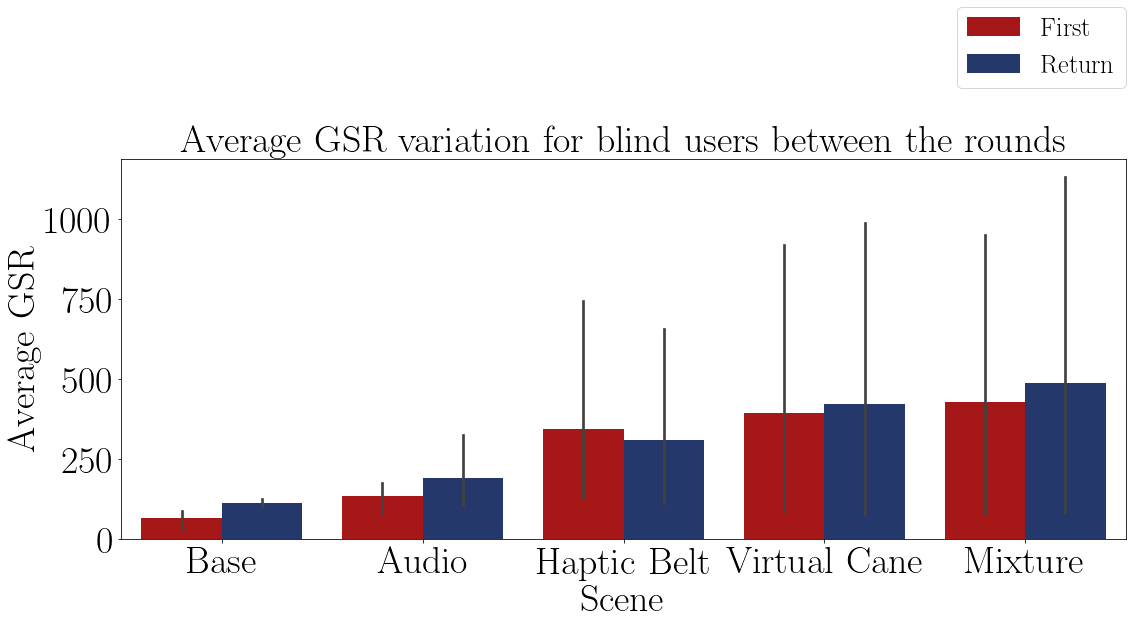
\includegraphics[width = 0.8\linewidth]{Resultados/GSR/Figuras/png/barplot_gsr_avg_5_scene_blind.png}
    \caption{Barplot of the average SDNN of the blind participants on each method.}
    \label{fig:barplot_gsr_avg_5_scene_blind}
\end{figure}

The Table \ref{tab:gsr_average_group_blind} presents the average GSR variation presented in the table \ref{tab:gsr_var_blind}. It shows that the "Audio" method presented the lesser GSR, that could be a combination of the fact that during the "Audio" method the hands was not used and that the participants felt less strange to the method, since it is based a common daily activity.


\begin{table}[!htb]
\centering
\caption{Average GSR variation by the blind participants}
\label{tab:gsr_average_group_blind}
\begin{tabular}{lrrrrr}
\toprule
{} &      Base &     Audio & \begin{tabular}[c]{@{}l@{}}Haptic\\ Belt\end{tabular} & \begin{tabular}[c]{@{}l@{}}Virtual\\ Cane\end{tabular} &  Mixture \\
Visual Condition &           &           &                                                       &                                                        &          \\
\midrule
Blind            &  141.10\% &  127.32\% &                                              244.62\% &                                               307.18\% &  344.366 \\
\bottomrule
\end{tabular}
\end{table}



The Figures \ref{fig:boxplot_gsr_avg_blind_scene} presents the distribution of the skin conductance on each method. It noticeable that the "Base" method has the lowest variation of all methods and that the presence of a haptic device increases its variance. The Figure \ref{fig:boxplot_gsr_avg_blind_rounds} presents the GSR grouped by the rounds and their are virtually the same.

\begin{figure}[!htb]
    \centering
    \begin{minipage}{0.45\textwidth}
        \centering
        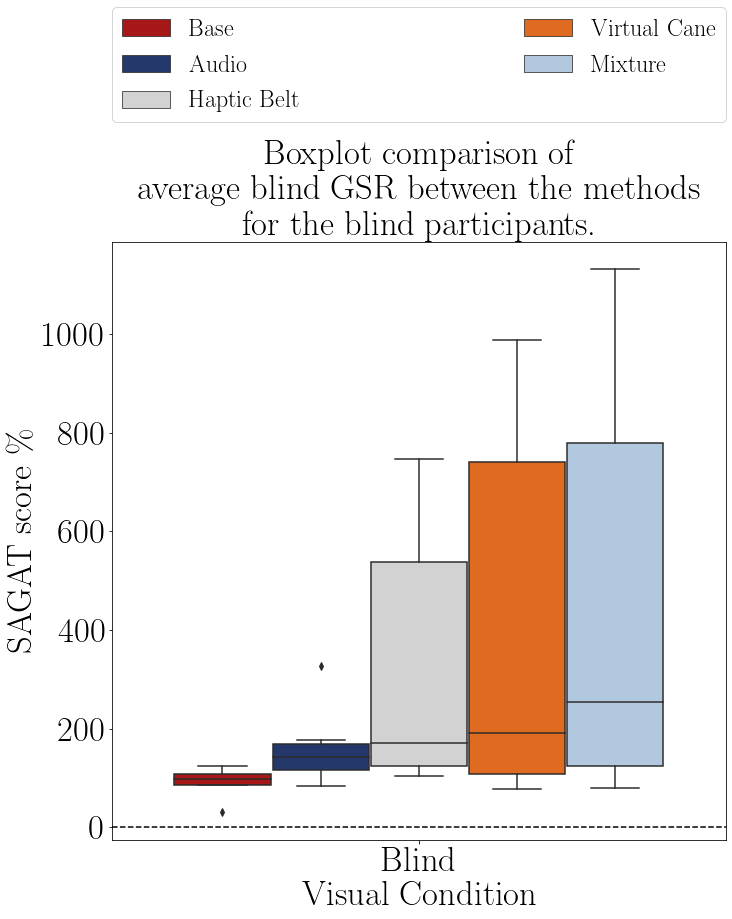
\includegraphics[width = 0.8\linewidth]{Resultados/GSR/Figuras/png/boxplot_gsr_avg_blind_scene.png}
        \caption{Boxplot of the GSR of the blind participants grouped by method.}
        \label{fig:boxplot_gsr_avg_blind_scene}
    \end{minipage}
    \begin{minipage}{0.45\textwidth}
        \centering
        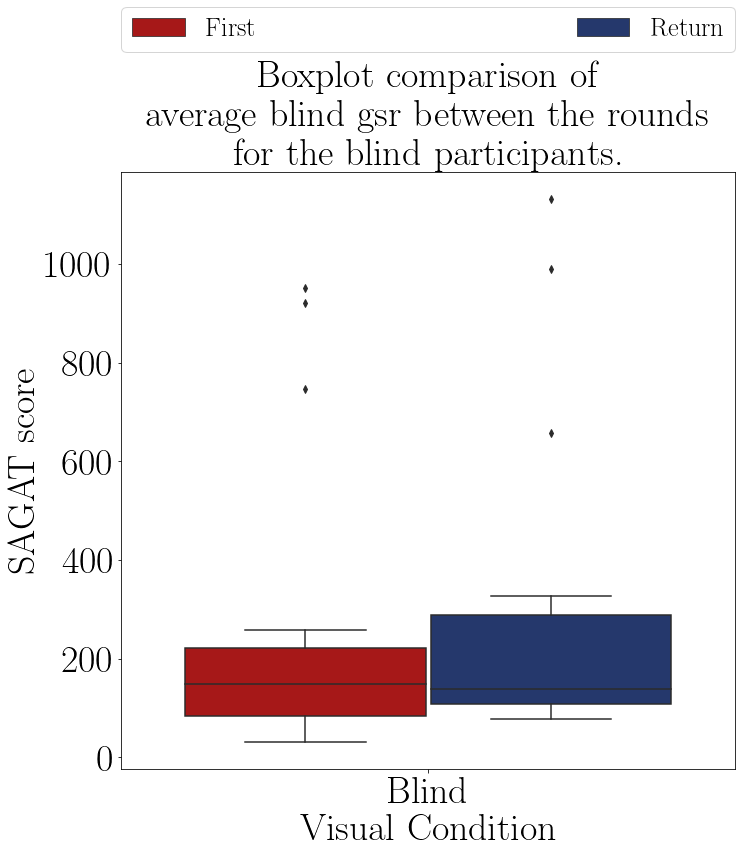
\includegraphics[width = 0.8\linewidth]{Resultados/GSR/Figuras/png/boxplot_gsr_avg_blind_rounds.png}
        \caption{Boxplot of the GSR of the blind participants grouped by round.}
        \label{fig:boxplot_gsr_avg_blind_rounds}
    \end{minipage}
\end{figure}

The Figures \ref{fig:qqplot_gsr_two_way} and \ref{fig:residplot_gsr_two_way} shows the distribution and variance of the Table \ref{tab:gsr_var_blind}. These Figures shows that the data are normally distributed but the participants had different  that the methods have a similar variance.
The Table \ref{tab:blocanova_gsr_two_way} shows the ANOVA test p-value of the heartbeat interval variance of the “blind” sample. The p-value indicates that there is no effect of any factor in the skin conductance.


\begin{table}[!htb]
\centering
\caption{Anova p-value for the mental demand average on each method for blinded users.}
\label{tab:blocanova_gsr_two_way}
\begin{tabular}{lrrrrl}
\toprule
               Source &  Squared sum &  DOF & Squared average &      F & \begin{tabular}[c]{@{}l@{}}P-Value \\ $(F_{0} > F)$\end{tabular} \\
\midrule
Participants (Blocks) &  1892069.020 &    3 &      630689.673 & 12.122 &                                                                  \\
         \    Methods &   301240.557 &    4 &       75310.139 &  1.447 &                                                            0.246 \\
          \    Rounds &      445.951 &    1 &         445.951 &  0.009 &                                                            0.927 \\
     \    Interaction &    10636.848 &    4 &        2659.212 &  0.051 &                                                            0.995 \\
   Experimental Error &  1404764.738 &   27 &       52028.324 &        &                                                                  \\
                Total &  3609157.113 &   39 &                 &        &                                                                  \\
\bottomrule
\end{tabular}
\end{table}



\begin{figure}[!htb]
    \centering
    \begin{minipage}{0.45\textwidth}
        \centering
        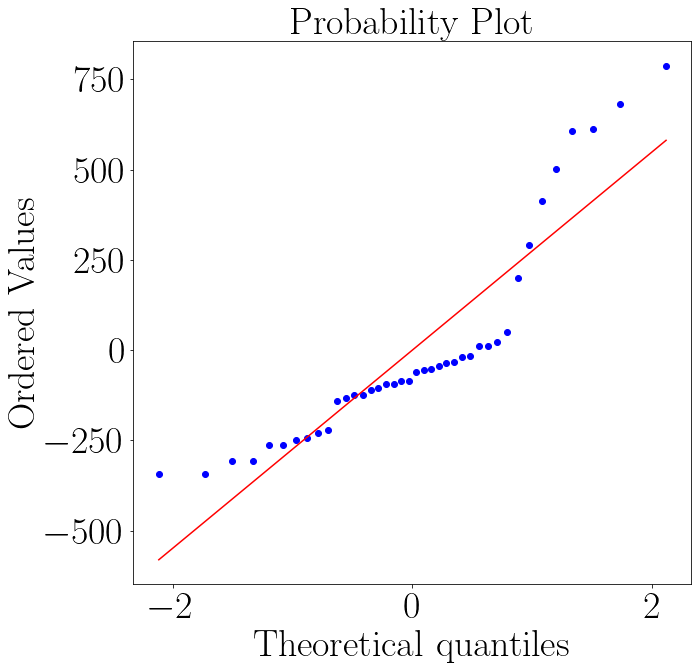
\includegraphics[width = 0.8\linewidth]{Resultados/GSR/Figuras/png/qqplot_gsr_two_way.png}
        \caption{QQ plot of the SDNN of the blind participants on each method.}
        \label{fig:qqplot_gsr_two_way}
    \end{minipage}
    \begin{minipage}{0.45\textwidth}
        \centering
        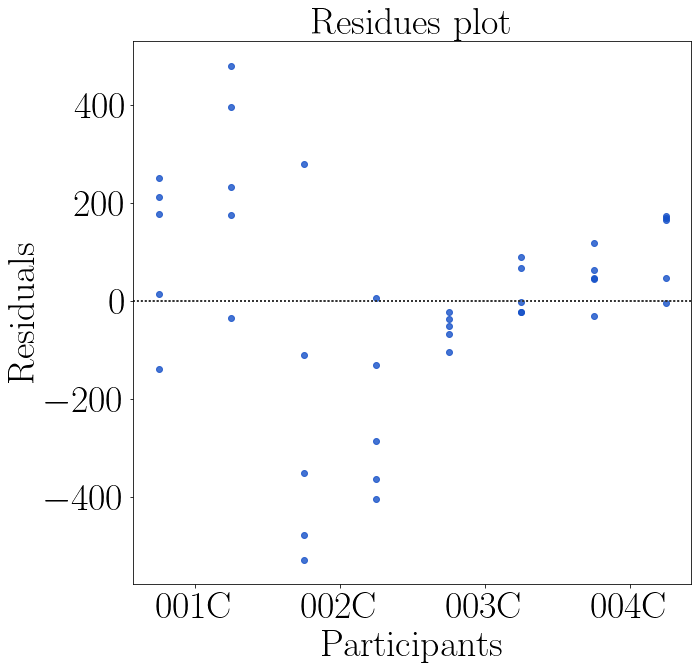
\includegraphics[width = 0.8\linewidth]{Resultados/GSR/Figuras/png/residplot_gsr_two_way.png}
        \caption{Residual plot of the SDNN of the blind participants on each method.}
        \label{fig:residplot_gsr_two_way}
    \end{minipage}
\end{figure}

%
\begin{table}[!htb]
\centering
\caption{Cross validation p-value for the mental demand average on each method for blinded users.}
\label{tab:lsd_gsr_two_way}
\begin{tabular}{rclr}
\toprule
      \multicolumn{3}{c}{Method} &                                           Analysis \\
\midrule
              Base & $X$ & Audio &                   $H_0 : \mu_{Base} = \mu_{Audio}$ \\
        Base & $X$ & Haptic Belt &         $H_1 : \mu_{Base} \ne \mu_{Haptic Belt}**$ \\
       Base & $X$ & Virtual Cane &        $H_1 : \mu_{Base} \ne \mu_{Virtual Cane}**$ \\
            Base & $X$ & Mixture &             $H_1 : \mu_{Base} \ne \mu_{Mixture}**$ \\
       Audio & $X$ & Haptic Belt &        $H_1 : \mu_{Audio} \ne \mu_{Haptic Belt}**$ \\
      Audio & $X$ & Virtual Cane &       $H_1 : \mu_{Audio} \ne \mu_{Virtual Cane}**$ \\
           Audio & $X$ & Mixture &            $H_1 : \mu_{Audio} \ne \mu_{Mixture}**$ \\
Haptic Belt & $X$ & Virtual Cane & $H_1 : \mu_{Haptic Belt} \ne \mu_{Virtual Cane}**$ \\
     Haptic Belt & $X$ & Mixture &      $H_1 : \mu_{Haptic Belt} \ne \mu_{Mixture}**$ \\
    Virtual Cane & $X$ & Mixture &         $H_0 : \mu_{Virtual Cane} = \mu_{Mixture}$ \\
\bottomrule
\end{tabular}
\end{table}



The Table \ref{tab:blocanova_gsr_two_way} does not prove that any method or round has some influence in the skin conductance variation, thus in the Mental Workload. Although, in the Figure \ref{fig:boxplot_gsr_avg_blind_scene} it is posible to notice that the "Base" and the "Audio" method have a different distribution. As it has already commented before, maybe the result of the anova test is a conseguence of a small sample size.

\FloatBarrier

